% easychair.tex,v 3.5 2017/03/15

\documentclass{easychair}

\usepackage{doc}

\newcommand{\easychair}{\textsf{easychair}}
\newcommand{\miktex}{MiK{\TeX}}
\newcommand{\texniccenter}{{\TeX}nicCenter}
\newcommand{\makefile}{\texttt{Makefile}}
\newcommand{\latexeditor}{LEd}


\title{Cybersecurity impacts at the beginning\\ of Covid-19 pandemic in Italy}

\author{
Marco R. A. Bozzetti\inst{1}
\and
    Fausto Spoto\inst{2}
\and
   Luca Olivieri \inst{2}
}

% Institutes for affiliations are also joined by \and,
\institute{
  President AIPSI\\
  Italian Chapter ISSA
\and
   University of Verona,
   Italy\\
   \email{\{fausto.spoto,luca.olivieri\}@univr.it}\\
 }

\authorrunning{M. Bozzetti, F.Spoto, L. Olivieri}

\titlerunning{Cybersecurity impacts at the beginning of Covid-19 pandemic in Italy}

\begin{document}

\maketitle

\begin{abstract}
%TODO
\end{abstract}


\section{Introduction}

The advent of the Covid-19 pandemic and the consequent lock-downs have led companies to face needs such as smart working, remotely work and digital business,
accelerating their digitalization efforts. As reported in \cite{Goasduff} by Gartner, a world's leading research and advisory company, before the pandemic crisis
most organizations moved their digital strategies forward at a steady pace, but during the Covid-19 pandemic there has been a significant increase in the 
development of digital products and services to maintain and accelerate customer engagement. However, the digitalization race has led to many cyber security issues
and the intensification of malicious cyber attacks around the world. In this scenario, Italy is an insteresting case of study because it is composed mostly from 
Small Medium Enterprises (SMEs) and therefore can highlight specific aspects instead of the various global views in which large companies have a greater influence.

\section{Digital Attacks Observatory}

The Digital Attacks Observatory (OAD)~\cite{OAD} is the only independent online survey in Italy about intentional digital attacks on IT systems of companies and public
bodies operating and in addition drawn up with the precious collaboration of the Italian Postal and Telecommunications Police. The OAD survey does not provide 
for a predefined set of respondents, but it allows potential interested parties full and free access to an online questionnaire, in a totally anonymous manner. 
Thanks to the number of responses collected and their balanced distribution between companies and public bodies of various sizes and belonging to various product 
sectors, the OAD survey provides a specific picture of the cyber-attacks in Italy.

\section{Data comparison}

OAD 2020 survey\footnote{The report is written in Italian, only the Executive Summary is in English: 186 A4 pages, 148 images and graphics, 11 Chapters
(147 A4 pages) and 9 Attachments (39 A4 pages)}~\cite{OAD_report_2020} took place during the Covid-19 pandemic, and it covered the entire 2019 and the first quarter 
of 2020, when in Italy the pandemic exploded. The data comparison of 2019 with these of the first quarter 2020, provided by the same pool of respondents, has a statistical relevance and provides a 
clear indication of the Covid pandemic on the intentional cyber-attacks in Italy. This pandemic has been the trigger for a wide range of cyberattacks, mainly 
caused by the sudden - and in part unprepared - passage of many to agile working from home and to a strong use of every type of IT service on Internet, mainly
derived by the mobility lockdowns imposed by the Italian Authorities. The emerged respondents’ pool covers all the product sectors, including Public Administrations,
even if the majority of the respondents’ companies belong to the ICT sector (30.8\%). The 2020 pool  is well balanced for the size of the organizations, in terms
of number of employees, between those below 250 and the largest ones. It must be taken into account that in Italy 99.91\%
\footnote{According to the last ISTAT census} %TODO: manca fonte/citazione
of enterprises are SMEs, under 250 employees, and 95\% are under ten employees. The OAD 2020 survey is therefore able to consider small and 
very small organizations, which are thee vast majority in Italy, and which are not normally considered in other cybersecurity surveys: 57.5\% of the OAD 2020 respondents
belong to structures with less than 250 employees, and of these 22.1\% under 10. The OAD questionaries refer for about half of the question to the cyber-attacks 
typologies and they main characteristics, if they have been relived. The other half of the questions refers to the technical and organizational security measures implemented
on the IT systems of the respondents. OAD therefore allows to contextualize the cyber-attacks with the cyber measures in production in each IT system considered. 
In fact, OAD 2020 provided a macro qualitative evaluation of the implemented measures (within the specific context of the company), in order to improve the motivation to 
complete the questionaries to all the potential anonymous respondents. The results of this macro evaluation is shown in fig. 1, which shows that more than $ 2/3 $ of the 
respondents has a good level of cybersecurity.

\begin{figure}
	\centering
		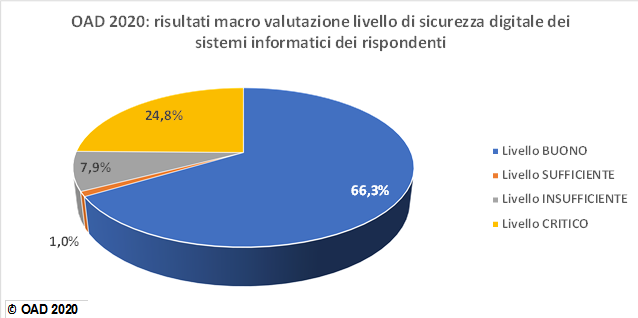
\includegraphics[width=1\textwidth]{pictures/fig1.png}
		\caption{}
		\label{fig:1}
\end{figure}

Fig. 2 compares the trend of the relived attacks from the beginning of the OAD survey in 2008: this comparison is only valid as a trend and not from a statistical point 
of view, due to the fact that the respondents pools year by year are different. Since 2007 to 2015, the “average trend” is focused about 40\% of the respondents that relived
cyber-attacks. (first red line in the figure). Since 2015 up to day, this average trend increased to 45\% of the respondents (second red line in the figure). In 2018 OAD 
reached the pick of relived attacks, and  for the first time  the \% of relived attacks is higher that the \% of the not relived.


\begin{figure}
	\centering
		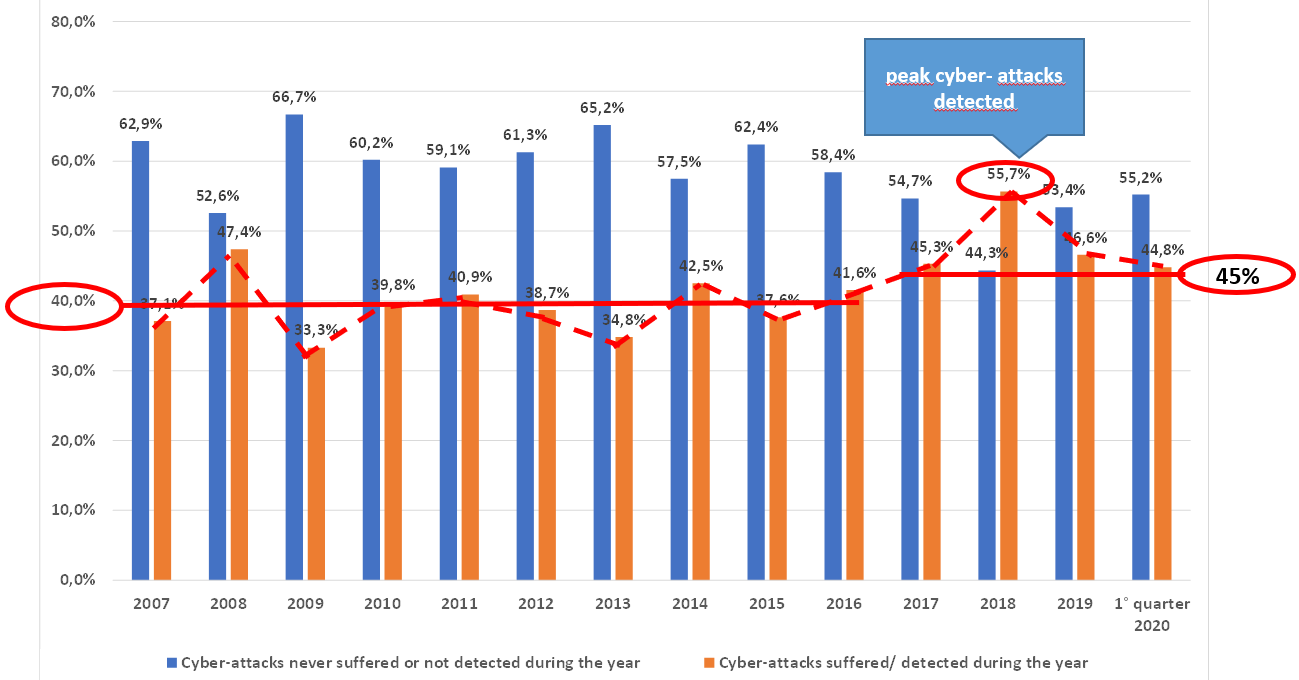
\includegraphics[width=1\textwidth]{pictures/fig2.png}
		\caption{}
		\label{fig:2}
\end{figure}


The dotted red line in the figure shows a wave shape: after a relative pick of attacks, the companies react hardening their cyber security, and the following year, normally, 
the relative pick in \% is lower that the previous one. After the biggest pick in 2018 as shown in fig.2,  2019 has a lower \%, and also for the first quarter 2020.
Only with the 2021 survey we will discover the \% for the whole 2020. The \%  in fig. 2 are lower than these expected.? We suggest to consider that:

\begin{itemize}
\item As shown in fig. 1, the majority of the respondents , in the OAD 2020 survey, has a good level of cyber security: about 30\% are of the ICT sector. 
Therefore the IT Systems can properly react to the cyber attacks. 

\item As pointed out before, 99,91\% of the companies in Italy are SME, and 95\% are under 10 employees. More r less is the same for the Public Administration (PA), 
the local ones in particular. The number of respondents in the 2020 OAD survey is 57,7\% for SME/small P, and of these 22,1\% are under 10 employees. 
The malicious hackers/crackers do not waist time for targeted attacks to very small realities.
\end{itemize}

Fig. 3 compares the cyber attacks relived in 2019 and in the first quarter of 2020 for the organization dimension. The black dotted line in the figure shows 
the “not” relieved attacks, and points out how it decrease from the very small to the very large organizations, in terms of numbers of employees. 


\begin{figure}
	\centering
		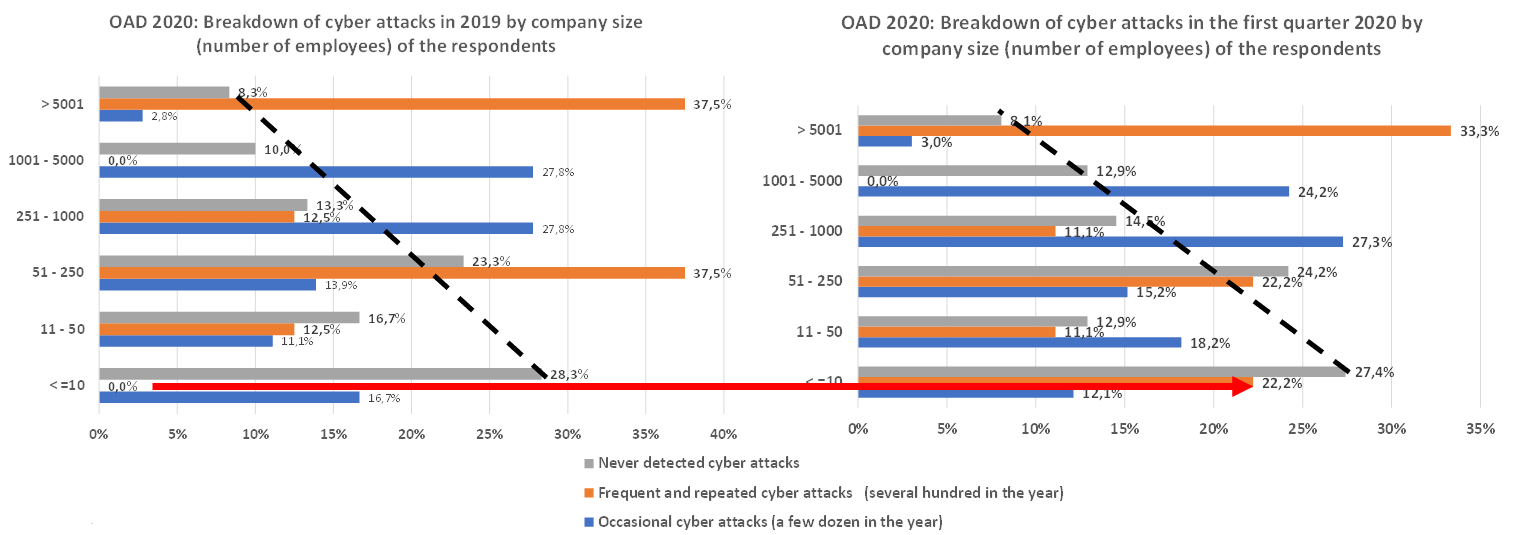
\includegraphics[width=1\textwidth]{pictures/fig3.png}
		\caption{}
		\label{fig:3}
\end{figure}


The figure confirms what already underlined before: the attackers try to hit the big structures, because with these it is more probable the realization of gains, even if illegal.
The comparison between the whole 2019 and the first quarter 2020 maintains the same logical trend. The only meaningful difference is for the frequent attacks relieved by the very
small organizations, up to 10 employees: 0\% in 2019 grows up to 22,2\% (see in fig. 3 the red line). Such a strong increase derives by the large utilization of e-baking and 
e-commerce services, with the related cyber attacks.


The impact of pandemic on the cyber security in Italy is also underlined by the data  provided by the Postal and Communications Police in fig. 4, that shows the situation for the
critical infrastructures, for the financial cyber crimes and for the cyber terrorism: and in particular for the financial cybercrimes. Fraudulent transactions in 2019 were blocked
for a total value of € 21.3 million and € 18 million were recovered; in the 1st quarter of 2020 fraudulent transactions for € 20.2 million were blocked, practically 
reaching in 4 months what was blocked in the 12 months of the previous year, and € 8 million recovered; an indicator of the growth in attacks on financial transactions and 
services due to the very large use of these online services caused by the mobility blocks imposed by the Covid-19 pandemic.


\begin{figure}
	\centering
		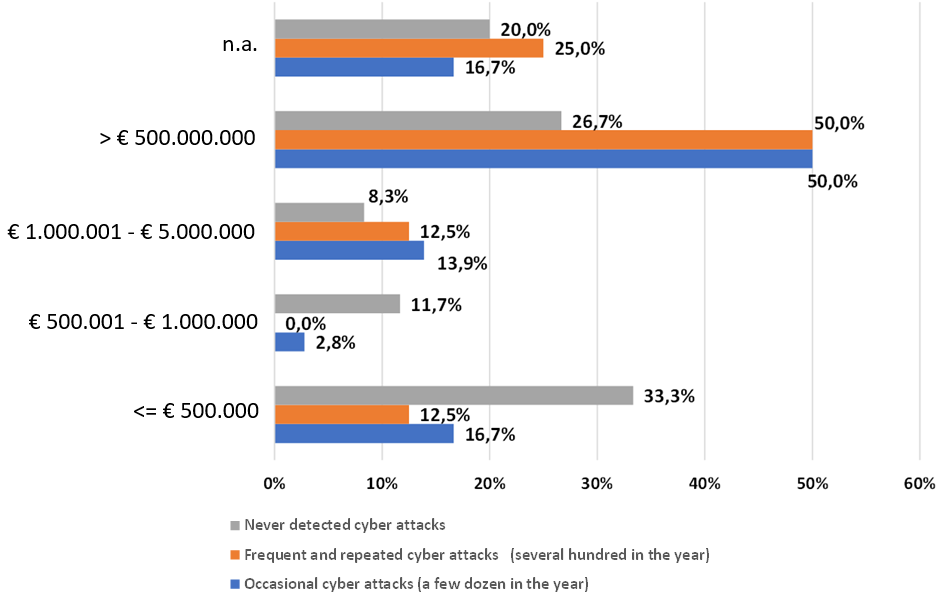
\includegraphics[width=1\textwidth]{pictures/fig4.png}
		\caption{}
		\label{fig:4}
\end{figure}


The type of attack (what is attacked) most widespread in both the considered periods is the one aimed at access control systems (IAA, Identification Authentication Authorization), 
with 34\% in 2019 and 28.2\% in the 1st quarter of 2020, as shown in fig. 5. As diffusion among the respondents, the other 14 types of attacks follow, decreasing by a few percentage
points among them, whose characteristics and impacts are detailed in the related paragraphs of the OAD 2020 report. Referring to the attack techniques (how to attack), all the seven
attacks families considered in the 2020 questionnaire are widely used in the various types of attacks, some times even simultaneously., as shown in fig. 6. The most widespread one,
as an average on the various attacks detected by the respondents’ pool, is the use of toolkits (rootkits, meta-exploits, etc.) for the identification and exploitation of vulnerabilities
on the target system of the attack, with a 38.8\%, followed by the well-known malicious and unauthorized collection of information (social engineering, phishing, etc.) with 34.6\% 
and the use of malicious code and scripts with 34.3%. The other considered techniques decrease with a few percentage points of difference between them. The impacts of the most 
critical attacks are analyzed for each attack type, as well as their possible motivations and the recovery times required by the most critical ones.


In the 2020 OAD survey, all these attacks’ characteristics vary for each type of attack, and the emerged results are described in the specific paragraphs dedicated to each attack 
type. At overall it emerges that:
\begin{itemize}
\item the impacts declared by the respondents are balanced between those irrelevant and / or easily resolvable with recovery in short time and at limited costs, and those very 
critical, which require expensive and long recovery actions, and that, in some cases, can cause business and customer loses; these two very different impact cases depend mainly 
on the security measures in place;

\item the motivations of the cyber-attacks are mainly of an economic nature, therefore done for fraud and blackmail: the widespread diffusion of ransomware in Italy is a clear 
confirmation of these motivations.
\end{itemize}


\begin{figure}
	\centering
		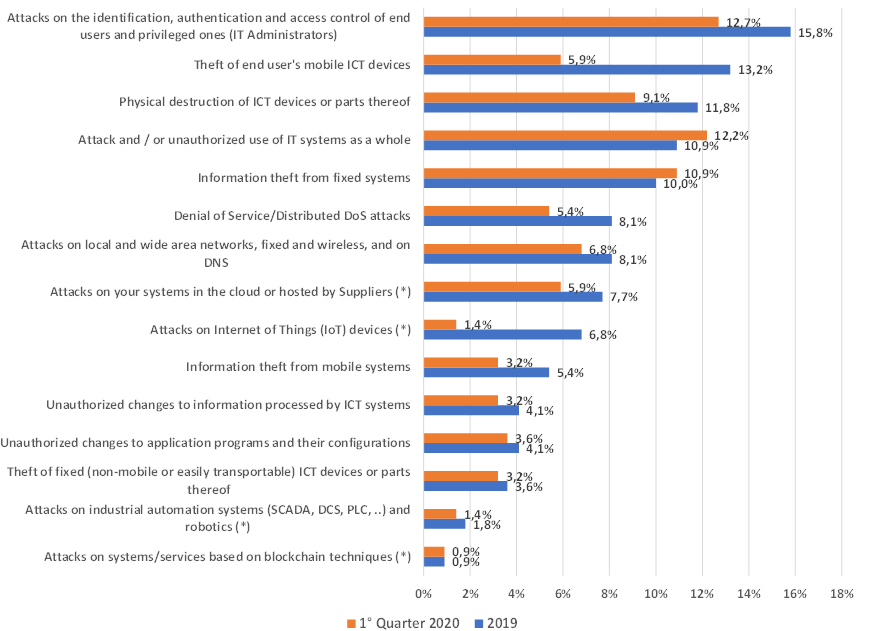
\includegraphics[width=1\textwidth]{pictures/fig5.png}
		\caption{}
		\label{fig:5}
\end{figure}
\begin{figure}
	\centering
		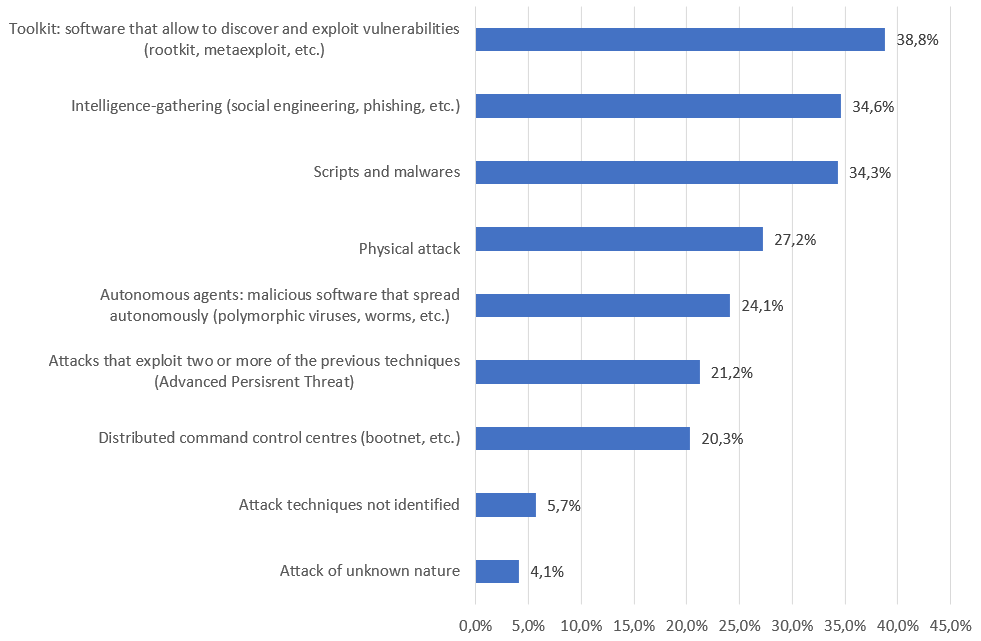
\includegraphics[width=1\textwidth]{pictures/fig6.png}
		\caption{}
		\label{fig:6}
\end{figure}
\begin{figure}
	\centering
		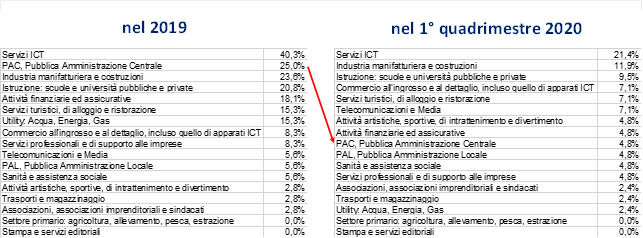
\includegraphics[width=1\textwidth]{pictures/fig7.png}
		\caption{}
		\label{fig:7}
\end{figure}
\begin{figure}
	\centering
		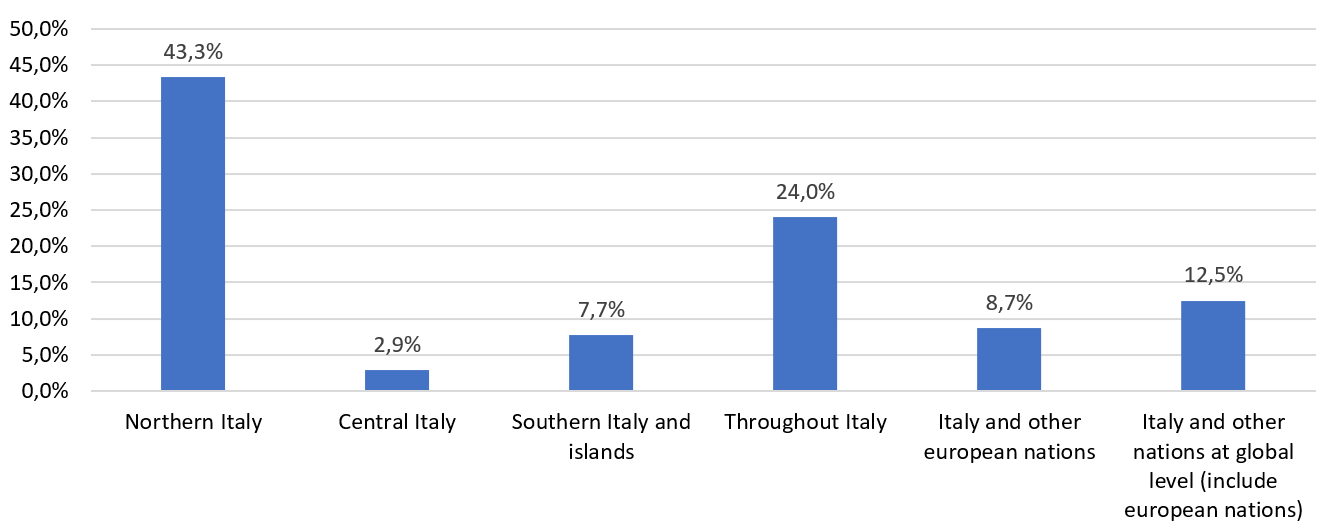
\includegraphics[width=1\textwidth]{pictures/fig8.png}
		\caption{}
		\label{fig:8}
\end{figure}


Fig. 8 shows the security measures considered in the 2020 questionnaire, subdivided in the technical ones, the organizational ones and  the management and governance ones. 
As pointed out in fig. 1, the Informatics Systems considered in the 2020 survey and their cybersecurity  are in the medium-high range and the emerged information  show a relevant 
improvement in both technical and organizational measures, in comparison to the previous surveys. Few of the considered Italian Informatics Systems are based on Data Centers in 
Italy, most of the respondents’ companies have medium-small Informatic Systems partly on premise and partly outsourced, with an increasing use of cloud services.
The high number of attacks detected in 2018, and the privacy obligations (GDPR) have certainly contributed to strengthening cyber security measures, and a further improvement 
comes from the growing use of cloud services, where usually there are high standard security measures. Organizational measures for cybersecurity, historically lacking and neglected
in Italy, have improved in terms of defining roles and separation of duties, of organizational policies and procedures, and of incidents management. These measures often are lacking
in small organizations, and in general the cybersecurity awareness and competence are low, and mainly at the top level of the public and private organizations. In Italy, there is 
still a long way to go in terms of cybersecurity continual training and awareness. A formal and bureaucratic approach for the organizational procedures is still prevalent, which 
once defined, often do not find a possible concrete applicability, periodic updates and operational tests: an emblematic example is represented by the Disaster Recovery plans for 
which, several times, the required alternative ICT resources to be used are not forecasted and allocated and there also not provided periodic exercises and simulations of the 
possible disasters. Cybersecurity management tools still have limited diffusion among the 2020 OAD respondents, in particular the most advanced ones based on artificial intelligence
techniques. The use of IoT, of industrial automation and of robotics systems, and also of systems based on blockchain techniques find a low number of respondents involved, which 
also derives from the limited percentage of their product sectors that should be the more interested in these systems: the manufacturing sectors, the logistics, the research and 
development centers and labs, the Local Public Administrations for territorial control, and so on. For these topics, the data that emerged from the survey are considered only as 
specific cases that contribute to the general values on the cyberattacks, but which cannot be still considered of reference at the Italian level.

\section{Conclusion}

The OAD 2020 survey highlights a situation of cyberattacks of various types but all technically of ian high complexity and sophistication, with a slightly increasing 
spread  in Italy  compared to the trend that emerged in the twelve years of OAD surveys, but lower than the peak of 2018. Despite the proliferation of cyberattacks to varying 
degrees related to the Covid-19 pandemic, in the first four months of 2020 the general spread of attacks is at similar values to those of 2019: to be verified with the next OAD 2021
if there will be changes to this trend.


The Italian reality, made up of a very large number of small and very small organizations, does not make our country one of the most attractive for cybercriminals, but cyber warfare
and massive attacks represent a growing and serious risk, as has already happened in part with the widespread of ransomware on computer systems whit a lack of or  with low 
cybersecurity  basic measures. OAD 2020 notes a clear improvement and strengthening of digital security measures, both technical and organizational, even if the most modern 
prevention, protection and management systems that use artificial intelligence techniques are still embryonic  in the respondents' basin.


The defense measures and techniques in use chase the increasingly sophisticated and smart evolution of attacks, but almost always late. The high density of vulnerabilities 
requires different approaches and new logics, with the aim of making all ICT systems interconnectable to the Internet intrinsically safe, by default and by design. But we are 
still a long way from this goal, and in order to decisively improve the concrete fight against continuous attacks and cybercrime, it is currently necessary to increase 
cybersecurity’ awareness and skills at all levels, an effective collaboration between the police at world level, and primarily a real and large usage of the professional ethics
 both of those involved (supply side) and both of those who decide (demand side) on cybersecurity.

\bibliographystyle{plain}
\bibliography{biblio}

\end{document}

